
\fancyhead[C]{Section 14.5}
\fancyhead[R]{\dayeleven}

\iftoggle{questions}{
\begin{center}{\large \textbf{Math 2551 Worksheet: Gradient and Directional Derivatives}}
\end{center}

\begin{enumerate}
	\item Use the contour diagram of the differentiable function f given below to decide if
	the specified directional derivative is positive, negative, or approximately zero.
	
	\begin{minipage}{0.3\linewidth}
		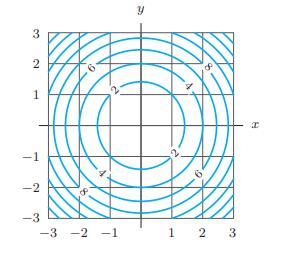
\includegraphics[scale=0.7]{contour_14_5.png}
	\end{minipage}
	\begin{minipage}{0.6\linewidth}	
		\begin{enumerate}
			\item At the point $(-2,2)$ in the direction $\bi$
			\item At the point $(0,-2)$ in the direction $\bj$
			\item At the point $(-1,1)$ in the direction $\bi +\bj$
			\item At the point $(-1,1)$ in the direction $-\bi+\bj$
			\item At the point $(0,-2)$ in the direction $\bi - 2\bj$
		\end{enumerate}
	\end{minipage}
	
	\item Let $f(x,y)=xy$.  Sketch the curve $f(x,y)= -4$ together with $\nabla f(2,-2)$ and the tangent line at $(2,-2)$. Then, find an equation for the tangent line.  What do you notice?
	
	
	\item Find the derivative of $g(x,y)= \dfrac{x-y}{xy+2}$ at $(1,-1)$ in the direction of $\langle 12, 5\rangle$.

	
	\item Suppose you are climbing a hill whose shape is given by the equation
	\[ z = 1000 - 0.005x^2-0.01y^2, \]
	where $x, y,$ and $z$ are measured in meters, and you are standing at a point with
	coordinates $(60, 40, 966)$. The positive $x$-axis points east and the positive $y$-axis
	points north.
	\begin{enumerate}
		\item If you walk due south, will you start to ascend or descend? At what rate?
		\item If you walk northwest, will you start to ascend or descend? At what rate?
		\item In which direction is the slope largest? What is the rate of ascent in that direction?
	\end{enumerate} 
	\item Let $f(x,y)=-x^2y+xy^2+xy$ and $P=(2,1)$.
	\begin{enumerate}
		\item Find the direction of maximal increase of $f$ at $P$.
		\item What is the maximum rate of change of $f$ at $P$?
		\item Find the direction of maximal decrease of $f$ at $P$.
		\item Find a direction $\bu$ such that $D_{\bu}f(P)=0$ (note this forces $\bu$ to be a unit vector!).
	\end{enumerate}
\end{enumerate}
}{}

\iftoggle{answers}{
\begin{center}{\large \textbf{Math 2551 Worksheet Answers:Gradient and Directional Derivatives}}
\end{center}

\begin{enumerate}

		\item 	\begin{enumerate}
			\item Negative
			\item Negative
			\item Approximately zero
			\item Positive
			\item Positive
		\end{enumerate}
		\item Tangent line: $-2(x-2)+2(y+2)=0$\\
		
	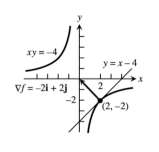
\includegraphics{14_5_sketch_soln.png}
		
		\item $D_{\bu}g(1,-1)=\dfrac{21}{13}$
		
		\item \begin{enumerate}
			\item Ascend at a rate of 0.8 vertical meters per horizontal meter
			\item Descend at a rate of $\sqrt{2}/10$ vertical meters per horizontal meter
			\item $\langle -0.6, -0.8\rangle$ is the direction of largest slope with rate of ascent 1 vertical meter per horizontal meter.
		\end{enumerate}
		\item 
		\begin{enumerate}
			\item $\langle -1/\sqrt{2},1/\sqrt{2} \rangle$
			\item $2\sqrt{2}$
			\item $\langle 1/\sqrt{2},-1/\sqrt{2} \rangle$
			\item $\langle 1/\sqrt{2},1/\sqrt{2} \rangle$
		\end{enumerate}
\end{enumerate}

}{}
\iftoggle{solutions}
{
Solutions go here in the same format.
}{}
